% \section{Instandhaltung und Support}

\section{Softwarebetrieb}

Diese Arbeit konzentriert sich auf Software, die sich in der Betriebsphase befindet. Gängige Software-Entwicklungszyklen und ihre Definition dieser Phase werden folgend beschrieben.

\subsection{Klassisches Vorgehen}

	\begin{wrapfigure}[14]{r}{0.45\linewidth}
		\centering
		\vspace{-\baselineskip}
		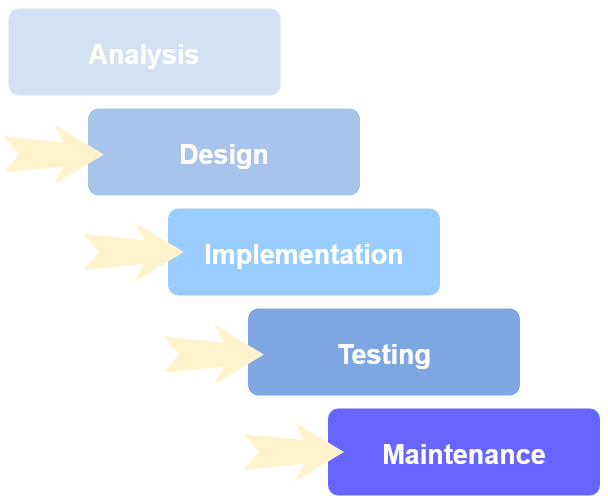
\includegraphics[width=\linewidth]{img/02_theorie/software-life-cycle.png}
		\caption{Lebenszyklus einer Software}
		\label{fig:software-development-life-cycle}
		\source{Eigene Darstellung von \cite{ASimulationModelWaterfallSoftware}}
	\end{wrapfigure}
	
	In vielen Modellen über den Lebenszyklus einer Software wird die Phase während der Betreibung oftmals ``Maintenance`` genannt \cite{ManagingTheComplexityOfWebSystemsDevelopment} \cite{ASimulationModelWaterfallSoftware}, in der Instandhaltung und Support den Alltag bestimmen. Sie ist nach Zelkowitz \etal \cite{PrinciplesOfSoftwareEngineeringAndDesign} für rund zwei Drittel der Entwicklungskosten verantwortlich, begründet durch exponentielle Steigung \cite{ExtremeProgrammingExplained}.
	
	Das Wasserfallmodell \cite{ASimulationModelWaterfallSoftware} sowie das V-Modell XT \cite{WaterfallVsVModelVsAgile} sehen vor, dass in dieser Phase die Software funktionstüchtig gehalten wird und dass die Anforderungen an die Software erfüllt sind. Bei nicht-erfüllten Anforderungen oder Fehlern, werden diese behoben. Jedoch ein kontinuierlicher Verbesserungsprozess ist in dieser Phase nicht vorgesehen.
	
%	Es werden immer bessere Methoden entwickelt, um Probleme in Software - oder auch Bugs - zu verringern. Jedoch erhöht sich zugleich die Komplexität von Software, was zur Ursache hat, dass es mehr Nährboden für Bugs gibt \cite{TrackingDownSoftwareBugsAnomalyDetection}. De-facto sind Bugs ein unvermeidbarer Bestandteil einer Software und müssen daher erwartet und gehandhabt werden \cite{TheMythicalManMonth}.
%	
%	Wenn nun ein Bug auffällt, sei es durch einen Nutzer oder auch zufällig einem Stakeholder, muss entschieden werden, ob dieser zu beheben ist. Wenn eine Behebung angestrebt wird, benötigt der Stakeholder meistens Rahmeninformationen \cite{WhatMakesAGoodBugReport} um den Bug ggf. zu reproduzieren und die Situation nachzuvollziehen. Desto mehr Verständnis der Stakeholder über das Problem erhält, desto schneller und präziser kann er die Ursache aufdecken. Die Ermöglichung der schnellen Verständnis über ein Problem, wird in dieser Arbeit \textbf{Nachvollziehbarkeit} genannt.

\subsection{Agiles Vorgehen}

	\begin{wrapfigure}[11]{l}{0.45\linewidth}
		\centering
		\vspace{-\baselineskip}
		\includegraphics[width=\linewidth]{img/02_theorie/devops-life-cycle.png}
		\caption{DevOps Toolchain}
		\label{fig:devops-life-cycle}
		\source{Wikimedia Commons \cite{DevOpsLifeCycle}}
	\end{wrapfigure}
	
	Bei agilen Ansätzen wird der Betrieb meist nicht abgegrenzt von der normalen Entwicklung. In dieser Phase werden weiterhin Anforderungen erhoben und diese Stück für Stück umgesetzt \cite{WaterfallVsVModelVsAgile}. Vorteilhaft dabei ist, dass auf neue Wünsche oder Auffälligkeiten sehr einfach reagiert werden kann. Es wird eine kontinuierliche Verbesserung angestrebt.
	
	Um den kontinuierlichen Entwicklungs- und Deploymentprozess reibungslos ablaufen zu lassen, werden Ansätze wie DevOps \cite{DevOps} verfolgt (vgl. \autoref{fig:devops-life-cycle}).